\documentclass{standalone}
\usepackage{tikz}
\usetikzlibrary{calc} % 坐标计算库
\usetikzlibrary{patterns} % 阴影填充库
\usepackage{pgfplots} % 绘图库
\usepgfplotslibrary{fillbetween} % 区域阴影
\pgfplotsset{compat=1.18} % 设置 pgfplots 版本
\usetikzlibrary{patterns.meta} % 图案库

% 常量声明
\newcommand{\xmin}{0}
\newcommand{\xmax}{7}
\newcommand{\ymin}{-11}
\newcommand{\ymax}{11}

\begin{document}

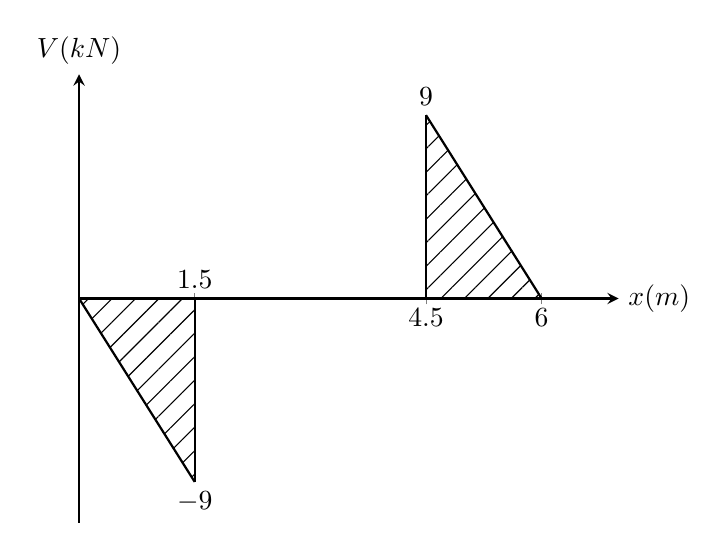
\begin{tikzpicture}
    % Shear Diagram
    \begin{axis}[
            axis lines=middle, % 学校式坐标轴
            axis line style={thick},
            xlabel={$x(m)$},
            xlabel style={right},
            ylabel={$V(kN)$},
            ylabel style={above},
            xtick={1.5,4.5,6},
            xticklabels={,,},
            xticklabel style={anchor=south, yshift=4pt},
            ytick=\empty,
            xmin=\xmin, xmax=\xmax,
            ymin=\ymin, ymax=\ymax,
        ]
        % 定义函数和x轴
        \addplot[name path=A, domain=0:1.5, thick] {-6*x};
        \addplot[name path=B, domain=1.5:4.5, thick] {0};
        \addplot[name path=C, domain=4.5:6, thick] {-6*(x-4.5)+9};
        \addplot[name path=AA, domain=0:1.5] {0};
        \addplot[name path=BB, domain=1.5:4.5] {0};
        \addplot[name path=CC, domain=4.5:6] {0};
        % 填充两者之间的区域
        \addplot[
            pattern={Lines[angle=45, distance=6pt]},
        ] fill between [of=A and AA];
        \addplot[
            pattern={Lines[angle=45, distance=6pt]},
        ] fill between [of=B and BB];
        \addplot[
            pattern={Lines[angle=45, distance=6pt]},
        ] fill between [of=C and CC];
        % 添加标识线或点
        % xtick
        \node at (axis cs:1.5,0) [above] {$1.5$};
        \node at (axis cs:4.5,0) [below] {$4.5$};
        \node at (axis cs:6,0) [below] {$6$};
        \node at (axis cs:1.5,-9) [below] {$-9$};
        \node at (axis cs:4.5,9) [above] {$9$};
        \draw[thick] (axis cs:1.5,0) -- (axis cs:1.5,-9);
        \draw[thick] (axis cs:4.5,0) -- (axis cs:4.5,9);
    \end{axis}

\end{tikzpicture}

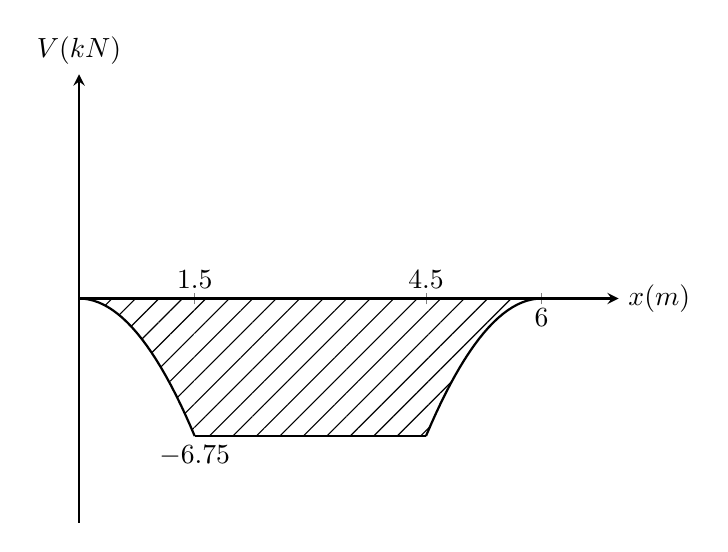
\begin{tikzpicture}
    % Moment Diagram
    \begin{axis}[
            axis lines=middle, % 学校式坐标轴
            axis line style={thick},
            xlabel={$x(m)$},
            xlabel style={right},
            ylabel={$V(kN)$},
            ylabel style={above},
            xtick={1.5,4.5,6},
            xticklabels={,,},
            xticklabel style={anchor=south, yshift=4pt},
            ytick=\empty,
            xmin=\xmin, xmax=\xmax,
            ymin=\ymin, ymax=\ymax,
        ]
        % 定义函数和x轴
        \addplot[name path=A, domain=0:1.5, thick] {-3*x^2};
        \addplot[name path=B, domain=1.5:4.5, thick] {-3*1.5*1.5};
        \addplot[name path=C, domain=4.5:6, thick] {-3*(x-4.5)^2+9*(x-4.5)-3*1.5*1.5};
        \addplot[name path=AA, domain=0:1.5] {0};
        \addplot[name path=BB, domain=1.5:4.5] {0};
        \addplot[name path=CC, domain=4.5:6] {0};
        % 填充两者之间的区域
        \addplot[
            pattern={Lines[angle=45, distance=6pt]},
        ] fill between [of=A and AA];
        \addplot[
            pattern={Lines[angle=45, distance=6pt]},
        ] fill between [of=B and BB];
        \addplot[
            pattern={Lines[angle=45, distance=6pt]},
        ] fill between [of=C and CC];
        % 添加标识线或点
        % xtick
        \node at (axis cs:1.5,0) [above] {$1.5$};
        \node at (axis cs:4.5,0) [above] {$4.5$};
        \node at (axis cs:6,0) [below] {$6$};
        \node at (axis cs:1.5,-6.75) [below] {$-6.75$};
    \end{axis}

\end{tikzpicture}

\end{document}